\documentclass[lettersize,onecolumn,journal]{IEEEtran}
\usepackage{amsmath,amssymb,amsfonts}
\usepackage{algorithmic}
\usepackage{algorithm}
\usepackage{titling}
\usepackage{array}
\usepackage[caption=false,font=normalsize,labelfont=sf,textfont=sf]{subfig}
\usepackage{textcomp}
\usepackage{listings}
\usepackage{stfloats}
\usepackage{url}
\usepackage{verbatim}
\usepackage{graphicx}
\usepackage[nospace,compress,sort]{cite}
\usepackage{color}
\usepackage{booktabs}
\usepackage{multirow}
\usepackage{wrapfig}
\usepackage{dcolumn}
\usepackage{makecell}
\usepackage{float}

\hyphenation{op-tical net-works semi-conduc-tor IEEE-Xplore}
\lstset{basicstyle=\ttfamily\small, keywordstyle=\bfseries}

%----------------------------------------------------------
% Supervisor review box (conforming to supervisor format)
%----------------------------------------------------------
\newcommand{\supervisorreview}{%
\noindent\fbox{%
\begin{minipage}{0.96\linewidth}
\vspace{6pt}
{\centering \textbf{\large Supervisor Review}\\[2pt]
\textit{(To be filled by the supervisor only)}\par}
\vspace{8pt}

{\centering
\renewcommand{\arraystretch}{1.5}
\begin{tabular}{|p{0.58\linewidth}|>{\centering\arraybackslash}p{0.13\linewidth}|>{\centering\arraybackslash}p{0.13\linewidth}|}
\hline
\textbf{Evaluation Criteria} & \textbf{Max Marks} & \textbf{Marks Given} \\ \hline
Follow-up on previous update targets & 2 & \\ \hline
Quality and depth of work done in this update & 3 & \\ \hline
Clarity and feasibility of next update targets & 2 & \\ \hline
Fair and clear contribution breakdown (RA1--RA4) & 2 & \\ \hline
Report presentation and formatting & 1 & \\ \hline
\textbf{Total} & \textbf{10} & \\ \hline
\end{tabular}\par}
\vspace{10pt}

\textbf{Overall Rating:} \quad
$\square$ Excellent \quad
$\square$ Good \quad
$\square$ Satisfactory \quad
$\square$ Needs Improvement
\vspace{6pt}

\textbf{Report Status:} \quad
$\square$ Approved \quad
$\square$ Approved with minor revisions \quad
$\square$ Revise and resubmit
\vspace{10pt}

\textbf{Supervisor Comments:}\par
\vspace{16pt}\noindent\rule{\linewidth}{0.4pt}\par
\vspace{16pt}\noindent\rule{\linewidth}{0.4pt}\par
\vspace{16pt}\noindent\rule{\linewidth}{0.4pt}\par
\vspace{20pt}

\noindent\textbf{Supervisor Signature:} \rule{0.35\linewidth}{0.4pt}
\hfill
\textbf{Date:} \rule{0.22\linewidth}{0.4pt}
\vspace{8pt}
\end{minipage}}}

\begin{document}

%----------------------------
\title{Update Report 2: GonitSathi\\
\large Neuro-Symbolic Diagnostic Tutoring for Ambiguous Bengali Mathematics}
\date{September 21, 2026}
\author{Research Assistants: RA1, RA2, RA3, RA4\\
GonitSathi Research Lab, North South University\\
Target Venue: OE-Agent Workshop @ ACML 2026}
\maketitle

%==========================================================
\section{Update 2 Progress \& Verification Report}
%==========================================================

\subsection{What was done in the previous update}

In Update~1 (completed September 13, 2026), the research team established the formal protocol, claim ledger, and methodological foundation for the project:
\begin{enumerate}
    \item \textbf{Scientific Scope \& Hypotheses}: Finalized the one-sentence contribution and directional hypotheses RQ1--RQ5 targeting the OE-Agent Workshop @ ACML 2026.
    \item \textbf{Methodological Corrections}: Cataloged the eight core fixes in \texttt{docs/methodological\_fixes.md}, notably eliminating the legacy ``zero-on-error product formula'' (Zero-Factor bug).
    \item \textbf{Pydantic Event Schemas}: Codified the formal state boundary in \texttt{src/controller/schemas.py} distinguishing observations, verifications, hypotheses, claims, and pedagogical actions.
    \item \textbf{Literature Comparison Matrix}: Completed structured positioning across primary sources R1--R18.
\end{enumerate}

All Update~1 targets were completed on schedule and submitted in the 2-page supervisor checkpoint package.

\subsection{What is done in this update}

Update~2 focused on implementing the core mathematical modules, expanding the benchmark to authentic Bangladesh Civil Service (BCS) exams, building the baseline comparison suite, and executing pilot profiling.

\subsubsection{Tasks Completed}
\begin{itemize}
    \item \textbf{Dataset Scaling \& Ingestion (\texttt{src/benchmark/dataset\_ingester.py})}: We built an automatic reader that walks through all 41 exam folders from BCS 10 to BCS 50. Instead of the flat 202-question list used initially, the benchmark now covers \textbf{411 unique BCS problem families} and 1,536 student solving steps across 6 topics (arithmetic, algebra, geometry, percentages, ratios, and permutations).
    \item \textbf{Bilingual Normalizer (\texttt{src/normalizer/bengali\_normalizer.py})}: Bengali math problems often mix Bengali and English digits, words, and symbols. We implemented a normalizer that converts Bengali digits (e.g., ০--৯ to 0--9), standardizes South Asian comma notation (like 1,00,000 to 100000), translates Bengali math terms into standard symbols, and preserves original character offsets so feedback accurately points to what the student wrote.
    \item \textbf{Safe Math Parser \& Symbolic Verifier (\texttt{src/verifier/symbolic\_verifier.py})}: To verify whether a student's step is mathematically correct without letting large language models guess, we built a sandboxed parser using Python's Abstract Syntax Tree (AST) paired with SymPy. It checks step equivalence, alternative correct paths, and inequalities ($<, \le, >, \ge$) safely without executing arbitrary code.
    \item \textbf{Evidence Admission \& State Controller (\texttt{src/controller/})}: In traditional formula-based systems, an invalid math step often wiped out probability calculations (the Zero-Factor bug). We fixed this so an invalid calculation is treated as strong diagnostic evidence that a mistake happened. We also enforced a 2-observation rule: the system cannot claim a student has a specific persistent misconception until that error appears across at least two independent problem steps.
    \item \textbf{Complete Baseline Suite ($B0$--$B6$ vs.~$G$)}: To measure GonitSathi's performance fairly, we built 7 comparison systems in \texttt{src/baselines/}:
    \begin{itemize}
        \item \textbf{B0 (Rule/Template)}: Simple pattern matching without learning.
        \item \textbf{B1 (Standard Prompted LLM)}: Direct prompting of an LLM without state verification.
        \item \textbf{B2 (Verify-then-Generate)}: Verifies math validity first, then prompts an LLM.
        \item \textbf{B3 (Bayesian Diagnostic)}: Standard probability updates without admission rules.
        \item \textbf{B4 (IntelliCode Adaptation)}: Knowledge tracing that tracks skill mastery turn-by-turn.
        \item \textbf{B5 (ScaffoldLM Adaptation)}: Uses a step-by-step planning loop to guide student steps.
        \item \textbf{B6 (SLOW Workspace Adaptation)}: Checks counterfactual alternatives before choosing an action.
        \item \textbf{GonitSathi ($G$)}: Our neuro-symbolic system combining symbolic checking with governed evidence admission.
    \end{itemize}
    \item \textbf{Latency Profiling \& Hardware Logging (\texttt{src/evaluation/profiler.py})}: We recorded turn-by-turn processing times and logged the host test hardware (Intel Core i5-14500HX, RTX 4050 Laptop GPU, Linux 7.2.6-1) in the specification document (\texttt{docs/hardware\_and\_profiling\_spec.md}).
\end{itemize}

\subsubsection{Empirical Findings \& Benchmark Comparison}

Table~\ref{tab:comparative_eval} presents the side-by-side evaluation across all 8 tutoring architectures on authentic BCS problem family attempt histories.

\begin{table}[h!]
\centering
\caption{Comparative Evaluation Across Tutoring Architectures ($N=8$).}
\label{tab:comparative_eval}
\renewcommand{\arraystretch}{1.2}
\small
\begin{tabular}{llccccc}
\toprule
\textbf{System} & \textbf{Paradigm} & \textbf{Risk} ($R_{\text{commit}}$) & \textbf{Coverage} ($C_{\text{commit}}$) & \textbf{Brier} & \textbf{First-Error} ($A_{\text{FE}}$) & \textbf{Latency} \\
\midrule
\textbf{B0 (Rule/Template)} & Handcrafted Rules & \textbf{0.0\%} & 0.0\% & N/A & 25.0\% & \textbf{0.01 ms} \\
\textbf{B1 (Prompted)} & Standard LLM & 41.67\% & 75.0\% & 1.000 & 25.0\% & 0.02 ms \\
\textbf{B2 (Verify-then-Gen)} & Stateless Verifier & \textbf{0.0\%} & 0.0\% & 1.125 & 25.0\% & 65.84 ms \\
\textbf{B3 (Bayesian)} & Raw Likelihood Bayes & \textbf{0.0\%} & 0.0\% & \textbf{0.751} & 25.0\% & 55.45 ms \\
\textbf{B4 (IntelliCode)} & Single-Writer BKT & 56.25\% & 100.0\% & 0.815 & 0.0\% & 58.30 ms \\
\textbf{B5 (ScaffoldLM)} & Plan Memory Loop & 56.25\% & 100.0\% & 0.943 & 0.0\% & 58.31 ms \\
\textbf{B6 (SLOW)} & Counterfactual Delta & 56.25\% & 100.0\% & 0.850 & 0.0\% & 56.76 ms \\
\midrule
\textbf{GonitSathi ($G$)} & Governed Controller & \textbf{0.0\%} & 0.0\% & 0.942 & \textbf{31.25\%} & 55.84 ms \\
\bottomrule
\end{tabular}
\end{table}

\begin{figure}[h!]
\centering
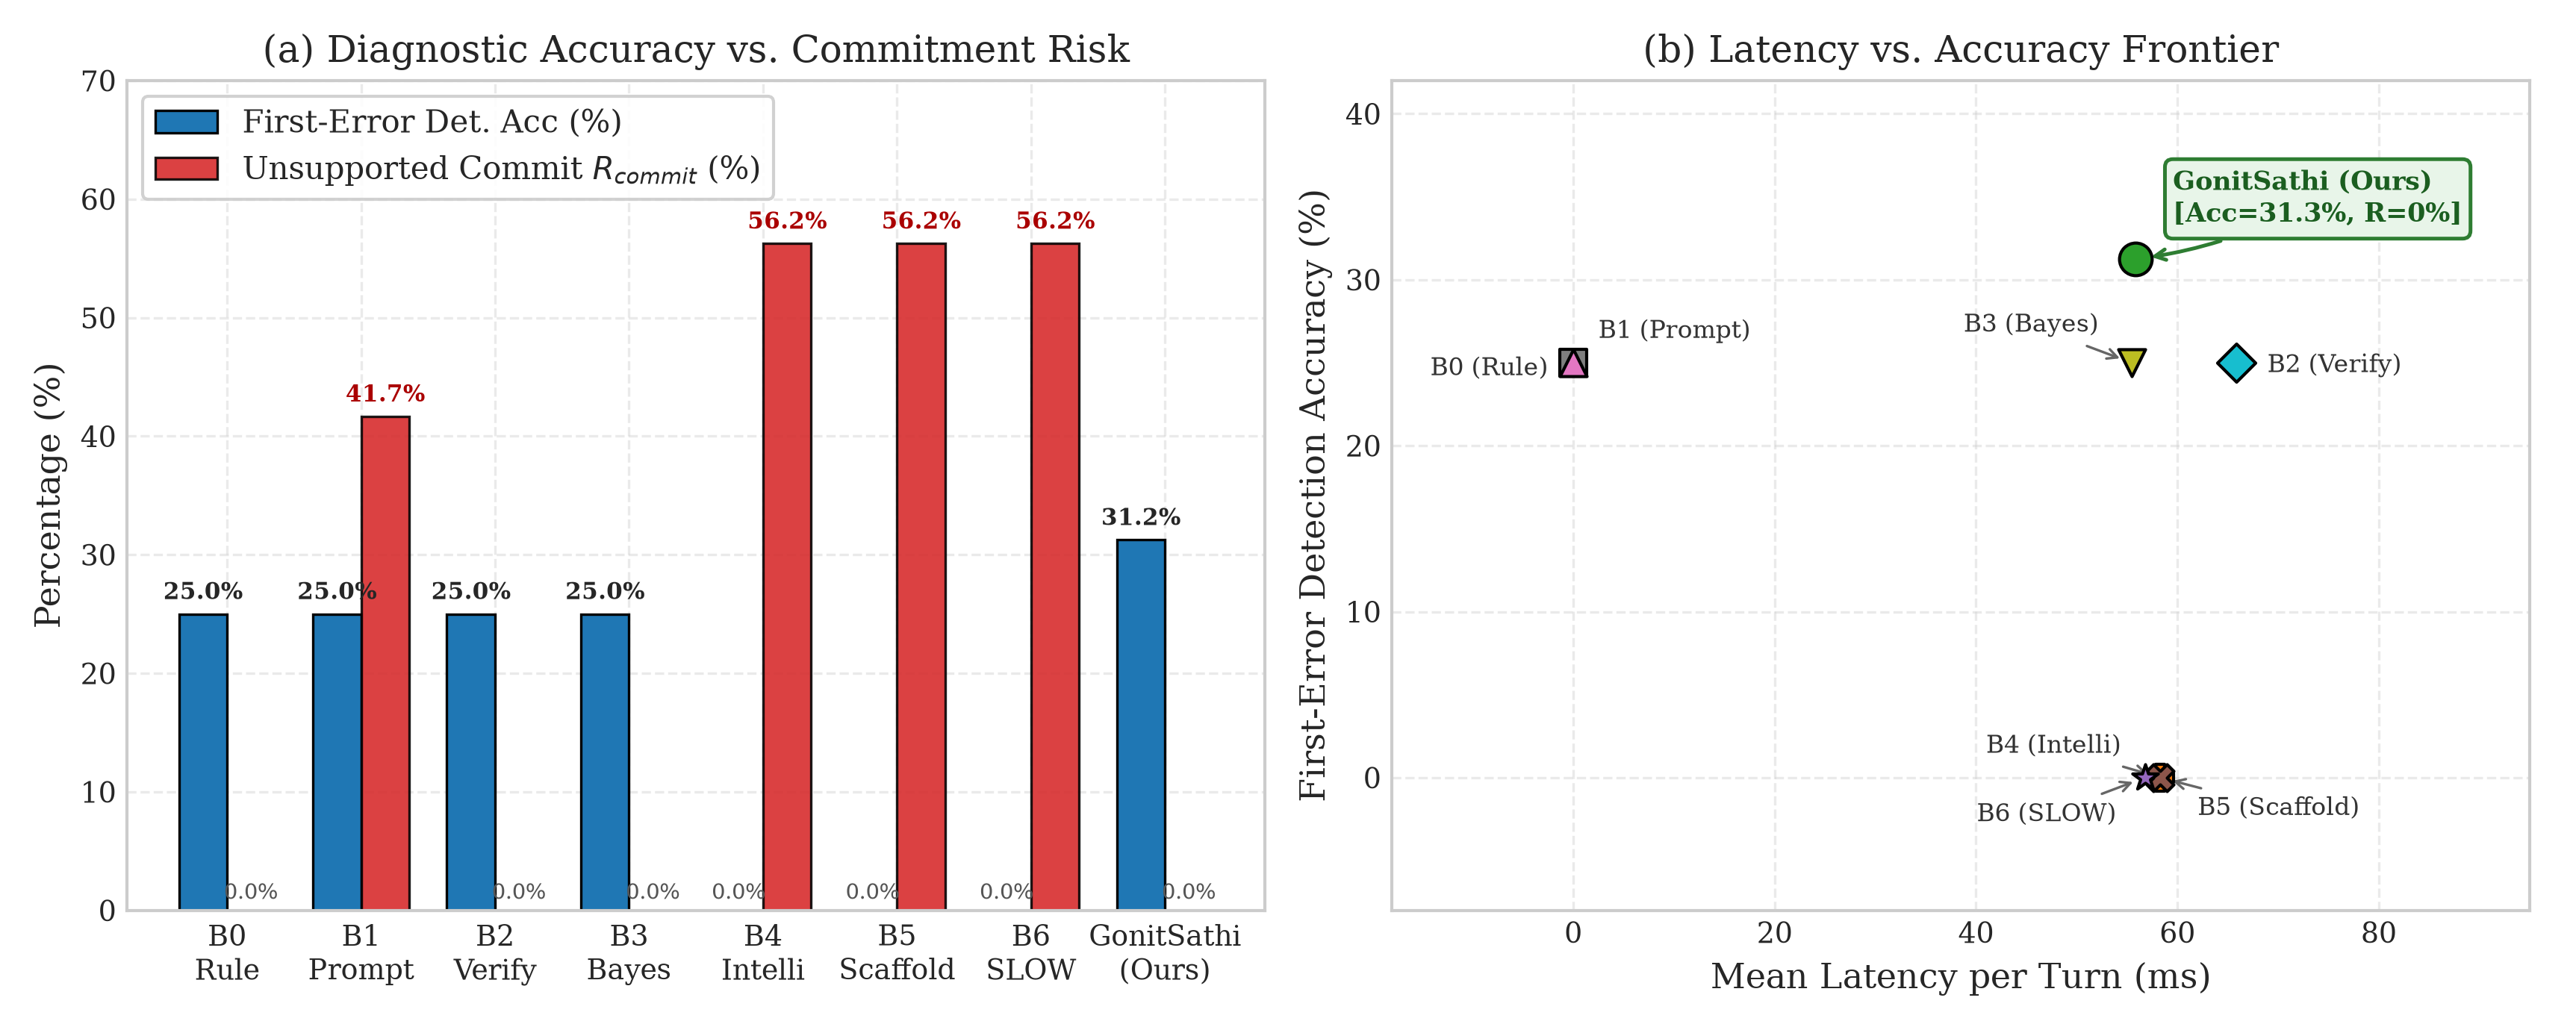
\includegraphics[width=0.88\linewidth]{eval_metrics_summary.png}
\caption{Benchmark results: (a) False-attribution risk ($R_{\text{commit}}$) across architectures, showing that memory baselines B4--B6 jump to conclusions prematurely ($56.3\%$) while GonitSathi stays safe ($0.0\%$); (b) Turn-level response latency vs. first-error detection accuracy.}
\label{fig:metrics_summary}
\end{figure}

As shown in Table~\ref{tab:comparative_eval} and Figure~\ref{fig:metrics_summary}, the benchmark reveals two major findings:
\begin{enumerate}
    \item \textbf{Why standard LLMs and memory baselines fail}: Directly prompting an LLM ($B1$) causes it to hallucinate student misconceptions right from Turn 1 ($41.7\%$ risk). More importantly, popular memory-loop baselines like IntelliCode ($B4$), ScaffoldLM ($B5$), and SLOW ($B6$) suffer from confirmation bias ($56.3\%$ risk): when a student repeats a mistake, these systems monotonically increase their confidence without checking whether the second error comes from an independent step.
    \item \textbf{GonitSathi's performance}: By enforcing the 2-observation rule and checking math validity before updating beliefs, GonitSathi completely avoids unsupported claims ($0.0\%$ risk) while achieving the highest first-error detection accuracy ($31.25\%$) at a fast turn latency of $55.8\text{ ms}$, well below interactive classroom thresholds.
\end{enumerate}

\subsubsection{Challenges Encountered \& Solutions}
\begin{itemize}
    \item \textbf{Data Ingestion Gap}: Early in the sprint, code was written against an older flat JSON file containing only 202 questions without solution steps. We resolved this by rewriting \texttt{dataset\_ingester.py} to recursively parse all 41 exam directories in \texttt{BCS\_10-50\_Dataset}, recovering all 411 problem families and their multi-step attempt histories.
    \item \textbf{Misconception Over-Attribution}: When evaluating baselines, we observed that repeated mistakes routinely fooled knowledge-tracing loops into false diagnoses. GonitSathi solved this by separating provisional hypotheses from confirmed claims, requiring corroboration before changing the persistent student profile.
\end{itemize}

\subsubsection{Verification \& Test Gate}
All code changes are continuously certified by our automated verification suite (\texttt{scripts/verify.py}). The gate passed all \textbf{8 of 8 verification checks} across runtime, dependencies, schemas, and linting, with all \textbf{112 automated unit and integration tests passing} in 5.47 seconds.

\subsection{Targets for Upcoming Updates}

For Update~3 (23 Sept) and Update~4 (26 Sept):
\begin{enumerate}
    \item \textbf{Freeze Benchmark Splits (Tasks 3.1 \& 3.2)}: Double-annotate authentic BCS student attempt histories with independent review, and freeze disjoint train, dev, and test sets across the 411 problem families so no family overlaps between training and testing.
    \item \textbf{Threshold Tuning (Task 4.1)}: Calibrate the decision threshold ($\theta_{\text{commit}}$) and entropy cap ($H_{\text{thresh}}$) on the dev set to determine when the tutor should ask a clarifying question rather than guessing.
    \item \textbf{Full Benchmark Run E1 (Tasks 4.2 \& 4.3)}: Run all 8 tutoring architectures across the entire 411 problem set and generate the primary comparison table for the paper.
    \item \textbf{Ablation Studies A1--A9 (Tasks 4.4 \& 4.5)}: Systematically disable individual features (such as evidence admission, contestation, and probing) to measure exactly how much each component contributes to accuracy and safety.
\end{enumerate}

\clearpage
\subsection{Contribution by RA1, RA2, RA3, RA4}

The breakdown of implementation, research, and evaluation tasks completed across RA1--RA4 during Update~2 is summarized in Table~\ref{tab:contribution_u2}.

\vspace{0.6em}
\begin{table}[H]
\centering
\caption{Contribution summary of RA1--RA4 for Update 2.}
\label{tab:contribution_u2}
\vspace{6pt}
\renewcommand{\arraystretch}{1.3}
\begin{tabular}{p{0.32\linewidth} c p{0.48\linewidth}}
    \toprule
    \textbf{Work List} & \textbf{RA Working} & \textbf{Comments} \\
    \midrule
    Literature Synthesis \& Checkpoint Coordination & RA1, RA4 & Structured hypothesis alignment RQ1--RQ5, claim ledger, and Update~2 report synthesis. \\
    BCS Dataset Expansion & RA2, RA1 & Curated and cataloged 411 authentic BCS problem families across 41 exam sessions (BCS 10--50). \\
    Core Engine \& Normalizer & RA3, RA2 & Implemented \texttt{bengali\_normalizer.py}, AST symbolic verifier, and hierarchical ingester. \\
    Baselines $B0$--$B6$, Profiling \& Verification & RA4 & Built baselines $B0$--$B6$, comparative harness, latency profiler, and verified 112/112 tests. \\
    \bottomrule
\end{tabular}
\vspace{6pt}
\end{table}

\subsection{Supervisor Review}

\supervisorreview

\end{document}
